\documentclass[english,floatsintext,man]{apa6}

\usepackage{amssymb,amsmath}
\usepackage{ifxetex,ifluatex}
\usepackage{fixltx2e} % provides \textsubscript
\ifnum 0\ifxetex 1\fi\ifluatex 1\fi=0 % if pdftex
  \usepackage[T1]{fontenc}
  \usepackage[utf8]{inputenc}
\else % if luatex or xelatex
  \ifxetex
    \usepackage{mathspec}
    \usepackage{xltxtra,xunicode}
  \else
    \usepackage{fontspec}
  \fi
  \defaultfontfeatures{Mapping=tex-text,Scale=MatchLowercase}
  \newcommand{\euro}{€}
\fi
% use upquote if available, for straight quotes in verbatim environments
\IfFileExists{upquote.sty}{\usepackage{upquote}}{}
% use microtype if available
\IfFileExists{microtype.sty}{\usepackage{microtype}}{}

% Table formatting
\usepackage{longtable, booktabs}
\usepackage{lscape}
% \usepackage[counterclockwise]{rotating}   % Landscape page setup for large tables
\usepackage{multirow}		% Table styling
\usepackage{tabularx}		% Control Column width
\usepackage[flushleft]{threeparttable}	% Allows for three part tables with a specified notes section
\usepackage{threeparttablex}            % Lets threeparttable work with longtable

% Create new environments so endfloat can handle them
% \newenvironment{ltable}
%   {\begin{landscape}\begin{center}\begin{threeparttable}}
%   {\end{threeparttable}\end{center}\end{landscape}}

\newenvironment{lltable}
  {\begin{landscape}\begin{center}\begin{ThreePartTable}}
  {\end{ThreePartTable}\end{center}\end{landscape}}




% The following enables adjusting longtable caption width to table width
% Solution found at http://golatex.de/longtable-mit-caption-so-breit-wie-die-tabelle-t15767.html
\makeatletter
\newcommand\LastLTentrywidth{1em}
\newlength\longtablewidth
\setlength{\longtablewidth}{1in}
\newcommand\getlongtablewidth{%
 \begingroup
  \ifcsname LT@\roman{LT@tables}\endcsname
  \global\longtablewidth=0pt
  \renewcommand\LT@entry[2]{\global\advance\longtablewidth by ##2\relax\gdef\LastLTentrywidth{##2}}%
  \@nameuse{LT@\roman{LT@tables}}%
  \fi
\endgroup}


  \usepackage{graphicx}
  \makeatletter
  \def\maxwidth{\ifdim\Gin@nat@width>\linewidth\linewidth\else\Gin@nat@width\fi}
  \def\maxheight{\ifdim\Gin@nat@height>\textheight\textheight\else\Gin@nat@height\fi}
  \makeatother
  % Scale images if necessary, so that they will not overflow the page
  % margins by default, and it is still possible to overwrite the defaults
  % using explicit options in \includegraphics[width, height, ...]{}
  \setkeys{Gin}{width=\maxwidth,height=\maxheight,keepaspectratio}
\ifxetex
  \usepackage[setpagesize=false, % page size defined by xetex
              unicode=false, % unicode breaks when used with xetex
              xetex]{hyperref}
\else
  \usepackage[unicode=true]{hyperref}
\fi
\hypersetup{breaklinks=true,
            pdfauthor={},
            pdftitle={The Effect of Definiteness and Accessibility of Recipient and Theme on NP Realization of Recipient Regarding Spoken and Written Corpora},
            colorlinks=true,
            citecolor=blue,
            urlcolor=blue,
            linkcolor=black,
            pdfborder={0 0 0}}
\urlstyle{same}  % don't use monospace font for urls

\setlength{\parindent}{0pt}
%\setlength{\parskip}{0pt plus 0pt minus 0pt}

\setlength{\emergencystretch}{3em}  % prevent overfull lines

\ifxetex
  \usepackage{polyglossia}
  \setmainlanguage{}
\else
  \usepackage[english]{babel}
\fi

% Manuscript styling
\captionsetup{font=singlespacing,justification=justified}
\usepackage{csquotes}
\usepackage{upgreek}



\usepackage{tikz} % Variable definition to generate author note

% fix for \tightlist problem in pandoc 1.14
\providecommand{\tightlist}{%
  \setlength{\itemsep}{0pt}\setlength{\parskip}{0pt}}

% Essential manuscript parts
  \title{The Effect of Definiteness and Accessibility of Recipient and Theme on
NP Realization of Recipient Regarding Spoken and Written Corpora}

  \shorttitle{The Effect of Definiteness and Accessibility}


  \author{Utku Turk\textsuperscript{1}}

  % \def\affdep{{""}}%
  % \def\affcity{{""}}%

  \affiliation{
    \vspace{0.5cm}
          \textsuperscript{1} Department of Linguistics, Boğaziçi University  }

  \authornote{
    Utku Turk, M.A.~student at the Department of Linguistics, Boğaziçi
    University.
  }


  \abstract{Up until today, the introspection procedure has been extensively used,
yet it was challenged to this degree only in the recent years. This
procedure allows linguists to gather observational data which has
empirical status to some extent. However, presenting a set of sentences
and expecting native judgments on these sentences can be quite
misleading. The sentences prepared by the researcher may lead
participants towards the researcher's bias unless the sentences and the
observational process is prepared thoroughly. Because corpora have
become widespread and are easy to analyze thanks to recent developments
incomputer science, many researchers have started to use daily
linguistic data without setting limitations. In this paper, a dataset
describing the details of the use of the dative structure in English in
the Switchboard corpus and the Treebank Wall Street Journal collection
has been used to account for the effects of the definiteness and the
accessibility of both the recipient and the theme on the realization of
the dative structure in English sentences.}
  \keywords{R, Ditransitive predicates, NP Realization, Definiteness, Accessibility \\

    
  }





\usepackage{amsthm}
\newtheorem{theorem}{Theorem}
\newtheorem{lemma}{Lemma}
\theoremstyle{definition}
\newtheorem{definition}{Definition}
\newtheorem{corollary}{Corollary}
\newtheorem{proposition}{Proposition}
\theoremstyle{definition}
\newtheorem{example}{Example}
\theoremstyle{definition}
\newtheorem{exercise}{Exercise}
\theoremstyle{remark}
\newtheorem*{remark}{Remark}
\newtheorem*{solution}{Solution}
\begin{document}

\maketitle

\setcounter{secnumdepth}{0}



\section{The Problem}\label{the-problem}

Big data and the advanced use of statistical tools allow us to answer
one of the intriguing questions: How do people form ditransitive
predicates and which factors determine the internal structure of the
verb phrase? Traditionally, these kinds of grammatical structures in
English have been analyzed from a more theoretical perspective and have
focused on native judgments, thus making it impossible to differentiate
the results from the researcher's own intuition. Moreover, many studies
have indeliberately shown that judgments are extremely problematic, and
most of the time these judgments come from an extremely restricted group
of people, a bell-jar around the researcher. Both of these problematic
situations are exemplified comprehensively by studies on dative
alternation (Bresnan, Cueni, Nikita, \& Baayen, 2007), which is the main
focus of this paper.

In this paper, the main question I asked and set out to find an
explanation for is as follows: What determines the phrasal structure of
ditransitive predicates in English? Throughout the paper and the data
analysis, two distinct characteristics of both the recipient and the
theme are used to identify when and why native speakers of English
choose to use prepositional dative structures. The independent variables
in this analysis are the definiteness of recipient, the definiteness of
theme, the accessibility of theme, and the accessibility of recipient.
With these variables, I aim to explain the effect of definiteness and
accesibility on dative structures in English sentences while accounting
for different corpora consisting of written and spoken media separately.

\section{The Dataset}\label{the-dataset}

The dataset used in this paper is from the R package languageR named
dative from the study by Bresnan et al. (2007). From this data set, I
have selected 6 columns to focus on and have described the properties of
the \(N = 3263\) observation in the Switchboard corpus and the Treebank
Wall Street Journal collection, spoken and a written media respectively.
The percentage of the spoken medium, Switchboard corpus, is 28.00\%,
which is also integrated into the model I will use in this paper. The
selected columns from this dataset form the basis of this paper's
analysis.

\section{Definitions}\label{definitions}

In this section, I will provide definitions for keywords I use
throughout the paper. According to Martin Haspelmath (2013),
ditransitive verbs are verbs with two arguments in addition to the
subject: a \enquote{recipient} or \enquote{addressee} argument, and a
\enquote{theme} argument. While the recipient is a special kind of goal
where the action is directed towards and which is associated with verbs
expressing a change in ownership, the theme is the element that
undergoes the action but does not change its state. (Dowty, 1991)

The definiteness of a phrase is determined with other elements that
precede it in the dataset. Certain determiners such as \emph{a/an, many,
some,} and \emph{either} mark an NP as indefinite whereas others,
including \emph{the, this, every,} and \emph{both} mark an NP as
definite. (Huddleston \& Pullum, 2002) In the dataset, accessibility
columns consist of three unique types of information: given, new, and
accessible. These columns identify the context accessibility of the
recipient and the theme. \emph{New} accessibility implies that the
element uttered is newly introduced to the discourse, \emph{given} means
that it was already uttered in the interaction, and \emph{accessible}
means even though it is not explicitly introduced to the discourse, it
is available in the discourse.

\section{What to Expect from Data}\label{what-to-expect-from-data}

Before starting to fit a model, I will demonstrate relevant averages and
interactions from the dataset graphically in order to show the relevant
relationships and to offer a better understanding of what to expect and
what not to expect.

\section{Plot of Marginal Effect of
Definiteness}\label{plot-of-marginal-effect-of-definiteness}

As can be seen in \emph{Figure 1}, the percentage of NP realization of
the recipient is affected significantly by both the definiteness of
theme and definiteness of recipient. While theme definiteness decreases
the chance of NP realization of the recipient, definiteness of the
recipient increases the percentage. However, the effect of the medium
the sentences are formed has an great effect on the differences between
the possible formations. While the NP realization of the recipient is
higher in the written medium, Treebank Wall Street, when the recipient
is definite, the effect of corpora slightly different when the recipient
is indefinite such that only the combination of indefinite recipient and
theme seems to be affected.

\begin{figure}

{\centering 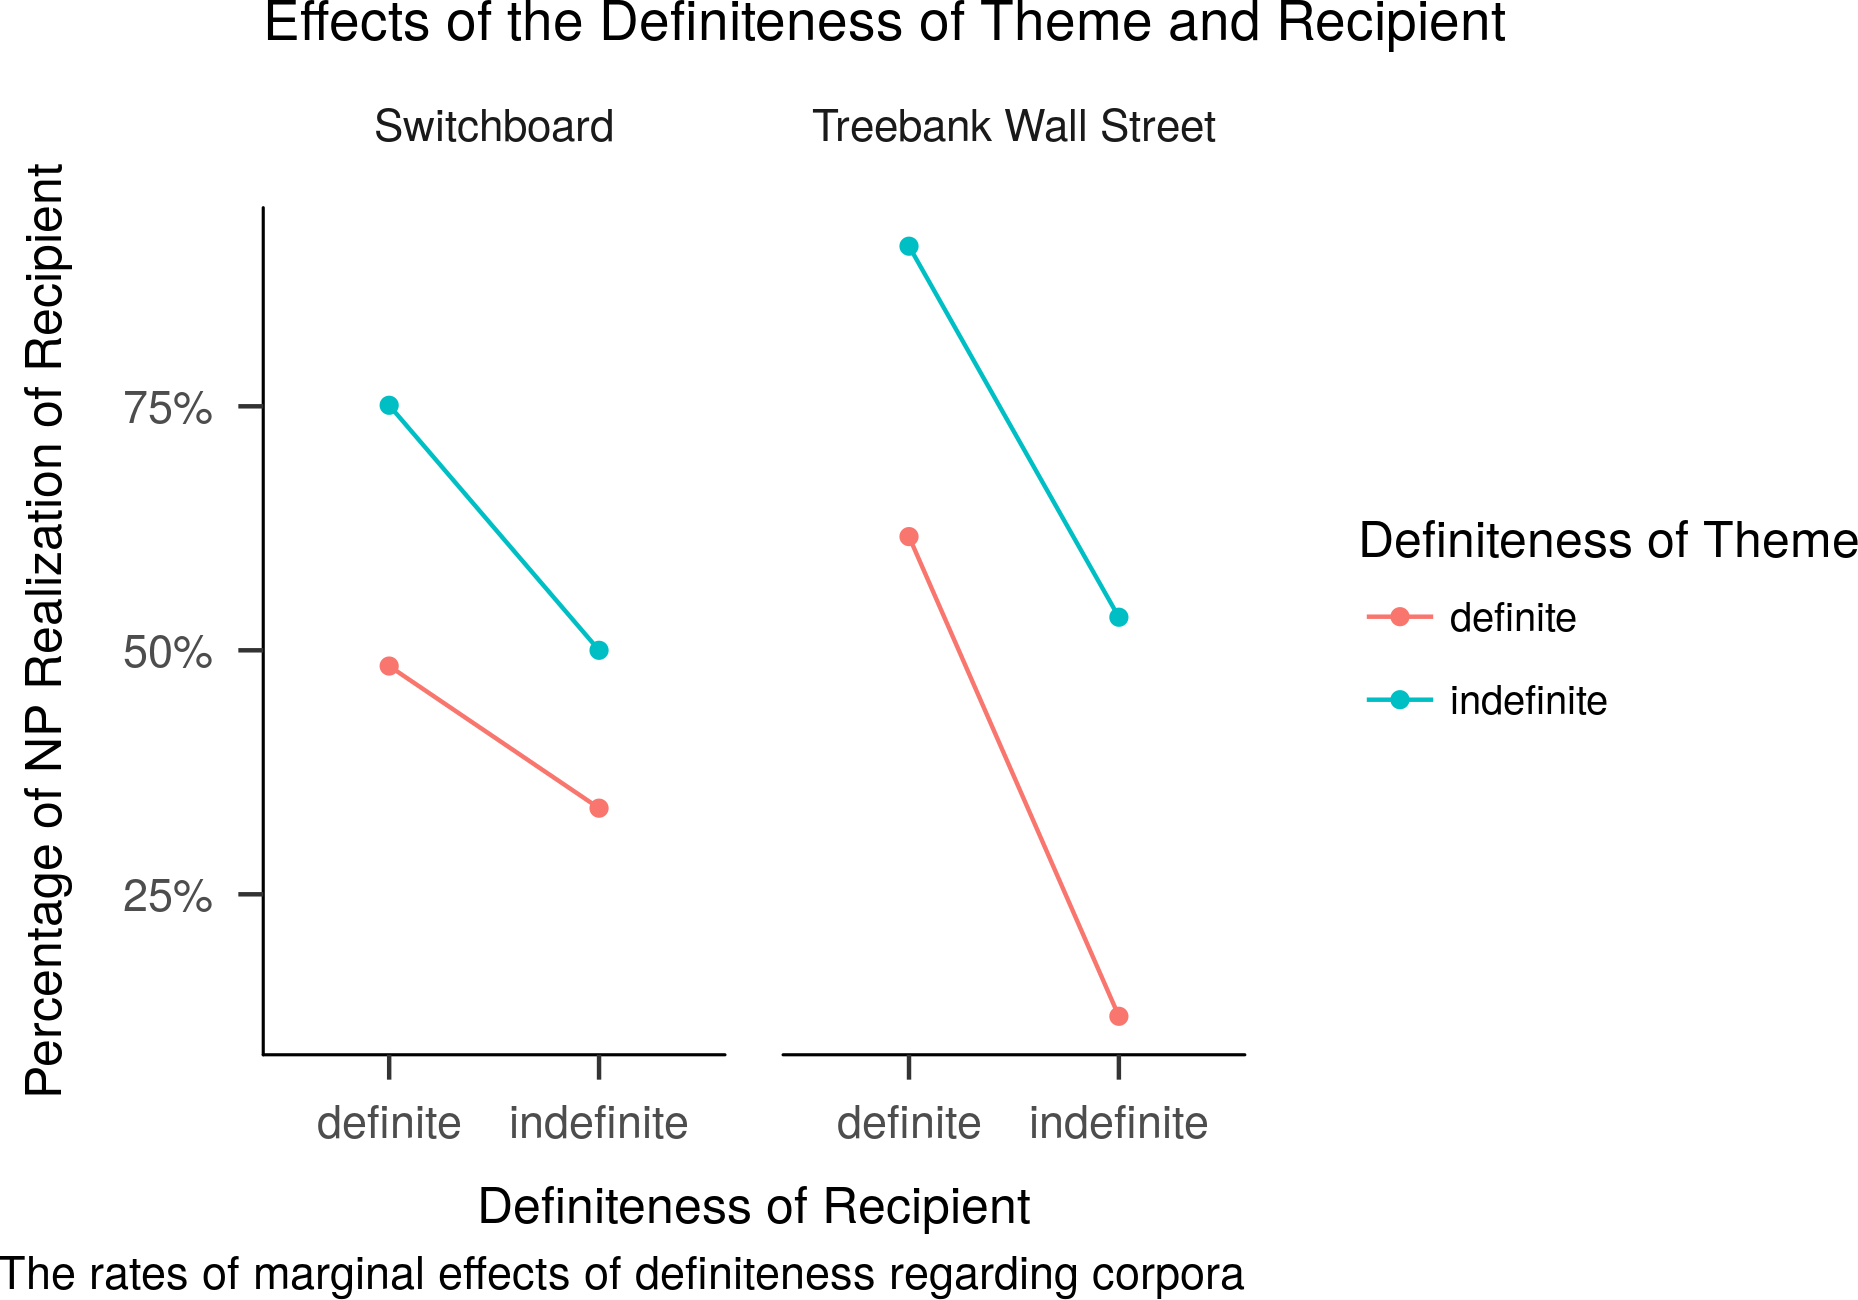
\includegraphics{papaja_files/figure-latex/unnamed-chunk-1-1} 

}

\caption{ }\label{fig:unnamed-chunk-1}
\end{figure}

\section{Plot of Marginal Effect of
Accessibility}\label{plot-of-marginal-effect-of-accessibility}

As for the \emph{Effects of Accessibility of Theme and Recipient}, while
the accessible and new theme do not really differ in terms of the
percentage of NP realization of recipient, the given theme definitely
and rather substantially decreases the NP realization tendency. The most
plausible scenario for NP Realization is when the theme is new, and the
recipient is given with the percentage of 57.80\%.

While the accessible and and new themes and recipients seem to behave
similarly, the differances between the averages of accessible recipient
in a spoken medium is slightly more pronounced.

\begin{figure}
\centering
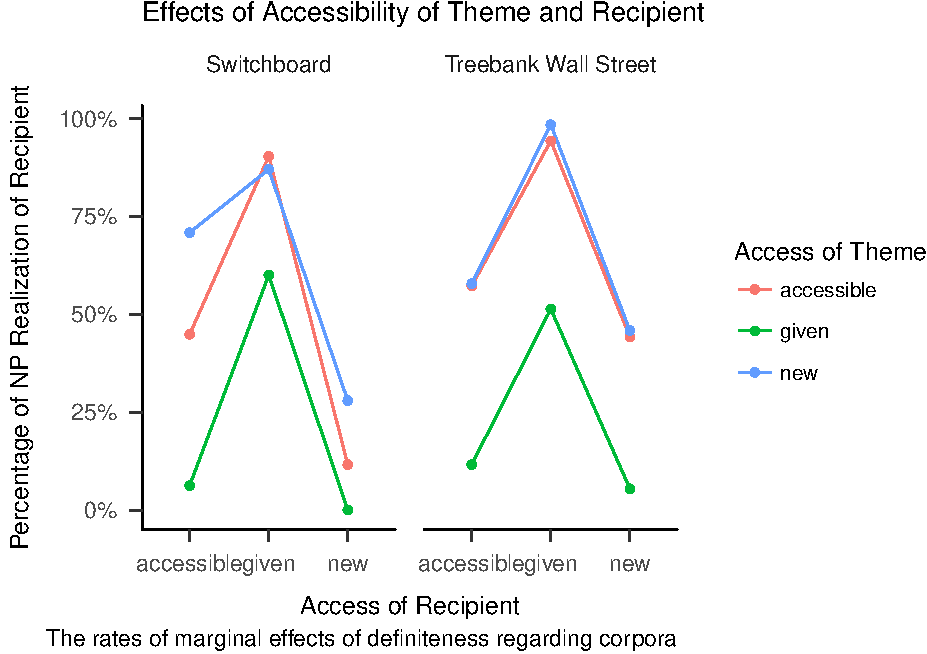
\includegraphics{papaja_files/figure-latex/acc_plots-1.pdf}
\caption{}
\end{figure}

\section{Plot of Marginal Effect of
Recipient}\label{plot-of-marginal-effect-of-recipient}

The effects related to the characteristics of the recipient are shown in
\emph{Figure 3}. It follows my first hypothesis which implied that there
would be a tendency toward an NP realization if the recipient was more
relevant in the discourse. Looking at \emph{Figure 3}, one can easily
argue that when the recipient is \emph{given} in the discourse and is
definite, English speakers put the recipient in the primary position,
making it a noun phrase rather than a prepositional phrase. Interaction
between the Access and the Definiteness of the recipient is not
non-existent, yet the definiteness of recipient effect is secondary at
best and negligible in the spoken corpus. However, accesible and new
indefinite recipients in the written corpus seem to behave quite
similarly in terms of the percentage of the NP realization of recipient.

\begin{figure}
\centering
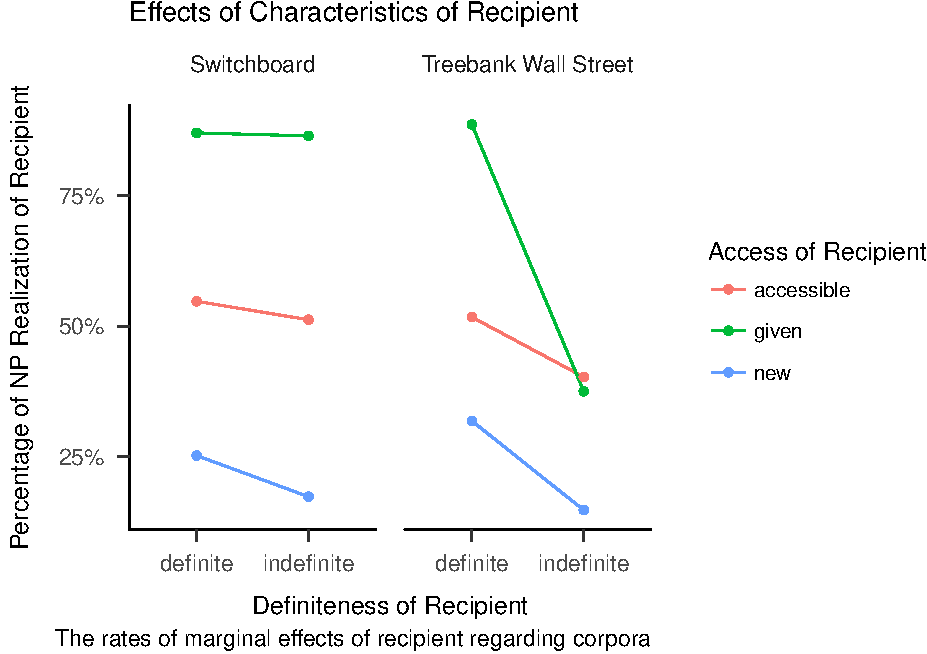
\includegraphics{papaja_files/figure-latex/rec_plots-1.pdf}
\caption{}
\end{figure}

\section{Plot of Marginal Effect of
Theme}\label{plot-of-marginal-effect-of-theme}

The percentage of NP realization of recipient in the data as a function
of the access and the definiteness of theme is shown in \emph{Figure 4}.
Among the four plots, this one clearly stands out. When the theme is
definite, the NP Realization of Recipient Hierarchy follows as such:
\emph{Accessible \textgreater{} New \textgreater{} Given}, which follows
my hypothesis. When the theme is indefinite, the effect of accessibility
seems to be almost disregarded. The percentages of NP realization of
recipient are 75\% and 94 \% in spoken and written media respectively
when the theme is given and indefinite. We would expect a lot less NP
realization of recipient from a given theme, yet the indefiniteness
characteristics outweights the accessibility of theme.

However, looking at the numbers in the accessible discourse, we can easy
infer that there is a somewhat fixed percentage. There must be an
interaction that tilts the percentages as such.

\begin{figure}
\centering
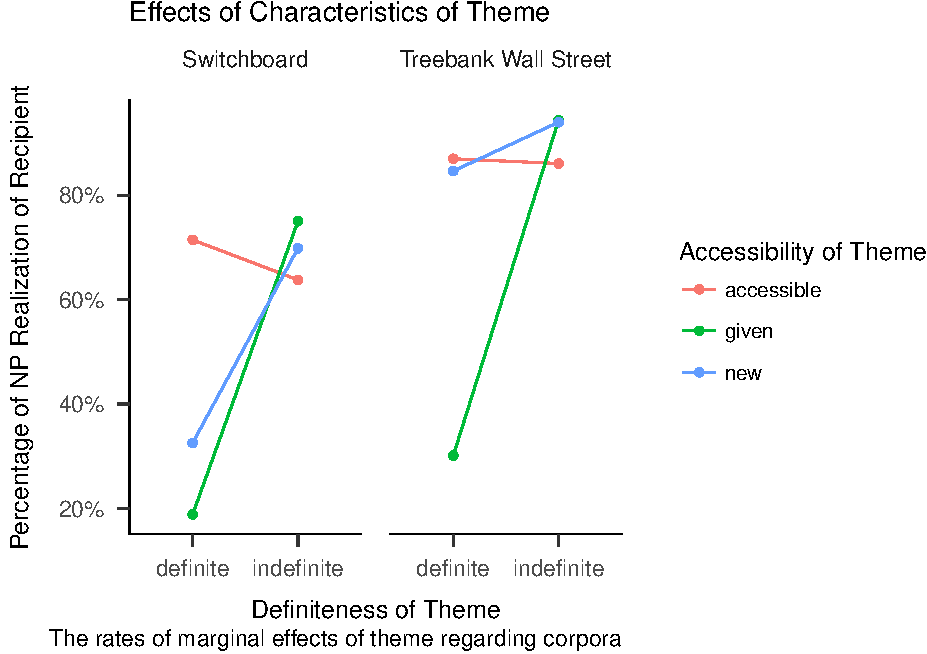
\includegraphics{papaja_files/figure-latex/thm_plots-1.pdf}
\caption{}
\end{figure}

\section{Hypothesis}\label{hypothesis}

After looking at the plots and the dataset, my hypothesis is that NP
realization of recipient increases with definite recipients and
indefinite themes. Also, the more familiar is the recipient, the more NP
realization of recipient we should see, and as the theme become more
familiar, I expect less NP realization of recipient. However, the
effects of corpora is more subtle, I definitely expect an effect between
spoken and written media, yet there is no clear cut move towards more or
less NP realization of recipient.

\section{Methods}\label{methods}

In the dataset, I included only 6 columns from the data, which are
discussed in the paper. The purpose of the paper is to identify the
effects of those variables; the rest is not included. Moreover, sum
contrasts are utilized for the definiteness of theme, the definitneess
of recipient, and the corpora while helmert contrasts are used for the
accessibility of recipient and the accessibility of theme in the model.

Apart from the relative information provided in the section titles
\textbf{Dataset}, I used R (Version 3.4.2; R Core Team, 2017) and the
R-packages \emph{bindrcpp} (Version 0.2; Müller, 2017), \emph{brms}
(Version 2.0.1; Bürkner, 2017), \emph{citr} (Version 0.2.0; Aust, 2016),
\emph{coda} (Version 0.19.1; Plummer, Best, Cowles, \& Vines, 2006),
\emph{dplyr} (Version 0.7.4; Wickham, Francois, Henry, \& Müller, 2017),
\emph{ggplot2} (Version 2.2.1; Wickham, 2009), \emph{knitr} (Version
1.17; Xie, 2015), \emph{languageR} (Version 1.4.1; Baayen, 2013),
\emph{lazerhawk} (Version 0.1.9; Clark, n.d.), \emph{magrittr} (Version
1.5; Bache \& Wickham, 2014), \emph{pander} (Version 0.6.1; Daróczi \&
Tsegelskyi, 2017), \emph{papaja} (Version 0.1.0.9655; Aust \& Barth,
2017), and \emph{Rcpp} (Eddelbuettel \& Balamuta, 2017; Version 0.12.14;
Eddelbuettel \& François, 2011) for the analyses, figures, and the
tables provided in the paper.

\section{Procedure and Data Analysis}\label{procedure-and-data-analysis}

Having explained the dataset, problem, and what to expect from the
dataset, we can advance to our model. First, the display of the model
used in the paper can be found below.
\[Realization_i \sim Bernoulli(\mu_i)\]
\[logit(\mu_i) = \alpha+\beta_{DoR}\times{DoR}+\beta_{AoR}\times{AoR}+\gamma_{i}\times{DoT_i}+\beta_{AoT}\times{AoT_i}+\beta_{corpora}\times{Corpora}+\gamma_k+\gamma_j\]
\[\gamma_i = \beta_{DoT}+\beta_{AoTDoT}AoT_i\]
\[\gamma_k = \beta_{corporaDoT}\times{Corpora\times{DoT}}\]
\[\gamma_j = \beta_{corporaDoR}\times{Corpora\times{DoR}}\] In the model
specified above, we used two linear models, which leads to a logistic
regression. The first line defines the likelihood function I used; it is
a Bernoulli distribution with logit link, which is specified in the
second line. The likelihood function consists of additive definition
integrated with another additive definition \(\gamma_i\) which is a
placeholder for the linear function that defines the slope between
\emph{Definiteness of Theme} and \emph{Access of Theme}. \emph{DoR, AoR,
DoT, AoT} stands for the definiteness of recipient, the accessibility of
recipient, the definiteness of theme, and the definiteness of theme,
respectively. Also, \(\gamma_k\) and \(\gamma_j\) represents the
interaction between the definiteness of theme and recipient,
respectively. Each \(\beta\) stands for the coefficient relevant to the
indeendent variable. This model is run through (Bürkner, 2017), which
sets improper flat priors by default. These priors are not changed.
Further analyses may be focused on identifying the relevant priors and
using them.

All models, interpretations, and functions are run through and
interpreted via Bayes Theorem. The primary underlying motivation behind
the utilization of Bayes Theorem is the fact that it provides me with
interpretable and reproducable answers without any fee except the
computational power of my processor. Even though the dataset's sample
size is rather large, reducing Bayes Theorem's importance to some
degree, describing and updating the probabilities of my hypothesis given
the evidence carry utmost importance for this paper. Since the Bayesian
Analysis complies with my likelihood function, the additive evidence,
and allows me to use a computationally-rich MCMC model, I ran such and
analysis and interpreted the output using a Bayesian approach.

\section{Results}\label{results}

\begin{table}[tbp]
\begin{center}
\begin{threeparttable}
\caption{\label{tab:summary}Inferential Statistics of NP Realization of Recipients}
\begin{tabular}{lllll}
\toprule
Covariate & \multicolumn{1}{c}{Estimate} & \multicolumn{1}{c}{Est.Error} & \multicolumn{1}{c}{Eff.Sample} & \multicolumn{1}{c}{Rhat}\\
\midrule
Intercept & -0.14 & 0.12 & 2,731.00 & 1.00\\
Theme Definiteness & 0.76 & 0.11 & 2,054.00 & 1.00\\
Theme Accessibility & 0.57 & 0.15 & 2,066.00 & 1.00\\
Theme Givenness & -0.19 & 0.07 & 2,595.00 & 1.00\\
Recipient Definiteness & -0.20 & 0.07 & 4,000.00 & 1.00\\
Recipient Accessibility & -1.09 & 0.07 & 3,956.00 & 1.00\\
Recipient Givenness & 0.77 & 0.05 & 4,000.00 & 1.00\\
Spoken Medium & 0.17 & 0.08 & 4,000.00 & 1.00\\
Definite Theme Accessibility & 1.04 & 0.15 & 2,139.00 & 1.00\\
Definite Theme Givenness & -0.05 & 0.07 & 2,716.00 & 1.00\\
Definite Theme in Spoken Corpus & -0.13 & 0.07 & 4,000.00 & 1.00\\
Definite Rec. in Spoken Corpus & 0.15 & 0.06 & 4,000.00 & 1.00\\
\bottomrule
\end{tabular}
\end{threeparttable}
\end{center}
\end{table}

The summary of our model is specified below in \emph{Table 1} without
credible intervals. Rows in the table shows names of covariates, their
estimates, Rhat value of the model, and effective sample size. The
\emph{Table 1} specifies that our model is converged succesfully.

\section{Discussion}\label{discussion}

\begin{table}[tbp]
\begin{center}
\begin{threeparttable}
\caption{\label{tab:discuss hpdis}Highest Posterior Density Intervals}
\begin{tabular}{lll}
\toprule
 & \multicolumn{1}{c}{lower} & \multicolumn{1}{c}{upper}\\
\midrule
Intercept & -0.31 & 0.06\\
Theme Definiteness & 0.57 & 0.92\\
Theme Accessibility & -0.15 & 0.12\\
Theme Givenness & 0.21 & 0.53\\
Recipient Definiteness & -0.31 & -0.07\\
Recipient Accessibility & -0.75 & -0.47\\
Recipient Givenness & -1.01 & -0.86\\
Spoken Medium & 0.06 & 0.31\\
Definite Theme Accessibility & -0.58 & -0.31\\
Definite Theme Givenness & 0.39 & 0.71\\
Definite Theme in Spoken Corpus & -0.25 & -0.02\\
Definite Rec. in Spoken Corpus & 0.05 & 0.26\\
lp & -1,163.27 & -1,155.66\\
\bottomrule
\end{tabular}
\end{threeparttable}
\end{center}
\end{table}

As we look at the \emph{Highest Posterior Density Intervals} with \%89
probability, only HPDIs not excluding 0 in their interval are our
\emph{Intercept} and \emph{Theme Accessibility} . As for the HPDIs,
\emph{Table 2} below shows that what we have predicted in the
\textbf{Hypothesis} section is strinkingly wrong for the definiteness of
theme and recipient. Theme definiteness affect the NP realizations of
recipient positively while recipient definiteness decreases the chance
of NP realization of recipient in English.

Upon looking at accessibility characteristics of the arguments, we see
that the difference between accessible and new theme is completely
negligible. It has almost a random effect on NP realization of recipient
with slight edge towards negative. Yet, \emph{Theme Givenness} affects
positively while \emph{Recipient Givenness} and \emph{Recipient
Accessibility} definitely have a negative effect in our model. Also, the
difference between accessible recipient and given recipient is not
negligible considering that they do not overlap in ther highest
posterior density intervals.

Moreover, English speakers tend to use more noun phrases for recipient
in dative structures in the \emph{Spoken Medium}, and definiteness of
theme in spoken discourse effects negatively whereas the interaction
between definite recipient and spoken corpus is headed towards positive.

As for the interaction between the characteristics of theme,
accessibility of theme when it is definite affects the NP realization of
recipient negatively. Thus, when we have an accessible theme which is we
are familiar with, we tend to use less NP. However, when the theme is
given in the speech we definitely use a lot more noun phrases for
recipients.

Looking from the whole picture, the model do not suggest exact opposite
of what we have predicted, nor it does not conform with our hypothesis.
It tends to conform to our hypothesis in interactions. However, the
inference from the definiteness scale is completely new to us.

We may need to change with which mentality we look at the data. the
reason behind the NP realization may not be in line with relevalance
principle, yet it may be about other hypothesis where people try to give
the new information as soon as possible eagerly and use the secondary
position as a safe zone. This question may also be related with the
length of recipient and theme, which we did not discuss in this paper.

All this confusing table shows us that further research is necessary. A
better model, another model with more variables, or crosslinguistic data
can shed light upon this question. Also, others paper regarding the
mental process behind sentence structures can help us on the way.

\pagebreak

\section{References}\label{references}

\setlength{\parindent}{-0.5in} \setlength{\leftskip}{0.5in}
\linespread{1}

\hypertarget{refs}{}
\hypertarget{ref-R-citr}{}
Aust, F. (2016). \emph{Citr: 'RStudio' add-in to insert markdown
citations}. Retrieved from \url{https://CRAN.R-project.org/package=citr}

\hypertarget{ref-R-papaja}{}
Aust, F., \& Barth, M. (2017). \emph{papaja: Create APA manuscripts with
R Markdown}. Retrieved from \url{https://github.com/crsh/papaja}

\hypertarget{ref-R-languageR}{}
Baayen, R. H. (2013). \emph{LanguageR: Data sets and functions with
``analyzing linguistic data: A practical introduction to statistics''.}
Retrieved from \url{https://CRAN.R-project.org/package=languageR}

\hypertarget{ref-R-magrittr}{}
Bache, S. M., \& Wickham, H. (2014). \emph{Magrittr: A forward-pipe
operator for r}. Retrieved from
\url{https://CRAN.R-project.org/package=magrittr}

\hypertarget{ref-Bresnan2007}{}
Bresnan, J., Cueni, A., Nikita, T., \& Baayen, R. H. (2007). Predicting
the dative alternation. \emph{Cognitive Foundations of Interpretation},
69--94.

\hypertarget{ref-R-brms}{}
Bürkner, P.-C. (2017). brms: An R package for bayesian multilevel models
using Stan. \emph{Journal of Statistical Software}, \emph{80}(1), 1--28.
doi:\href{https://doi.org/10.18637/jss.v080.i01}{10.18637/jss.v080.i01}

\hypertarget{ref-R-lazerhawk}{}
Clark, M. (n.d.). \emph{Lazerhawk: Miscellaneous functions mostly
inspired by synthwave}. Retrieved from \url{m-clark.github.io}

\hypertarget{ref-R-pander}{}
Daróczi, G., \& Tsegelskyi, R. (2017). \emph{Pander: An r 'pandoc'
writer}. Retrieved from \url{https://CRAN.R-project.org/package=pander}

\hypertarget{ref-Dowty1991}{}
Dowty, D. R. (1991). Montague's General Theory of Languages and
Linguistic Theories of Syntax and Semantics. In (pp. 1--36).
doi:\href{https://doi.org/10.1007/978-94-009-9473-7_1}{10.1007/978-94-009-9473-7\_1}

\hypertarget{ref-R-Rcpp_b}{}
Eddelbuettel, D., \& Balamuta, J. J. (2017). Extending extitR with
extitC++: A Brief Introduction to extitRcpp. \emph{PeerJ Preprints},
\emph{5}, e3188v1.
doi:\href{https://doi.org/10.7287/peerj.preprints.3188v1}{10.7287/peerj.preprints.3188v1}

\hypertarget{ref-R-Rcpp_a}{}
Eddelbuettel, D., \& François, R. (2011). Rcpp: Seamless R and C++
integration. \emph{Journal of Statistical Software}, \emph{40}(8),
1--18.
doi:\href{https://doi.org/10.18637/jss.v040.i08}{10.18637/jss.v040.i08}

\hypertarget{ref-Huddleston2002}{}
Huddleston, R. D., \& Pullum, G. K. (2002). \emph{The Cambridge Grammar
of the English Language} (p. 1842). Cambridge University Press.
Retrieved from
\href{http://www.cambridge.org/tr/academic/subjects/languages-linguistics/grammar-and-syntax/cambridge-grammar-english-language\%7B/\#\%7DXkWUSrQepi4REuRv.97}{http://www.cambridge.org/tr/academic/subjects/languages-linguistics/grammar-and-syntax/cambridge-grammar-english-language\{\textbackslash{}\#\}XkWUSrQepi4REuRv.97}

\hypertarget{ref-MartinHaspelmath2013}{}
Martin Haspelmath. (2013). Ditransitive Constructions: The Verb 'Give'.
Retrieved from \url{http://wals.info/chapter/105}

\hypertarget{ref-R-bindrcpp}{}
Müller, K. (2017). \emph{Bindrcpp: An 'rcpp' interface to active
bindings}. Retrieved from
\url{https://CRAN.R-project.org/package=bindrcpp}

\hypertarget{ref-R-coda}{}
Plummer, M., Best, N., Cowles, K., \& Vines, K. (2006). CODA:
Convergence diagnosis and output analysis for mcmc. \emph{R News},
\emph{6}(1), 7--11. Retrieved from
\url{https://journal.r-project.org/archive/}

\hypertarget{ref-R-base}{}
R Core Team. (2017). \emph{R: A language and environment for statistical
computing}. Vienna, Austria: R Foundation for Statistical Computing.
Retrieved from \url{https://www.R-project.org/}

\hypertarget{ref-R-ggplot2}{}
Wickham, H. (2009). \emph{Ggplot2: Elegant graphics for data analysis}.
Springer-Verlag New York. Retrieved from \url{http://ggplot2.org}

\hypertarget{ref-R-dplyr}{}
Wickham, H., Francois, R., Henry, L., \& Müller, K. (2017). \emph{Dplyr:
A grammar of data manipulation}. Retrieved from
\url{https://CRAN.R-project.org/package=dplyr}

\hypertarget{ref-R-knitr}{}
Xie, Y. (2015). \emph{Dynamic documents with R and knitr} (2nd ed.).
Boca Raton, Florida: Chapman; Hall/CRC. Retrieved from
\url{https://yihui.name/knitr/}






\end{document}
